Supplementary material for chapter \ref{chap:loy} and its corresponding manuscript: {\bf Loss of chromosome Y leads to down regulation of {\it KDM5D} and {\it KDM6C} epigenetic modifiers in clear cell renal cell carcinoma}.


%% Create counter for supp figs ("S1" etc)
\setcounter{figure}{0}
\renewcommand{\thefigure}{S\ref{chap:loy}.\arabic{figure}}
\setcounter{table}{0}
\renewcommand{\thetable}{S\ref{chap:loy}.\arabic{table}}

\section*{Supplementary Tables}

\begin{table}[ht]
  \centering
  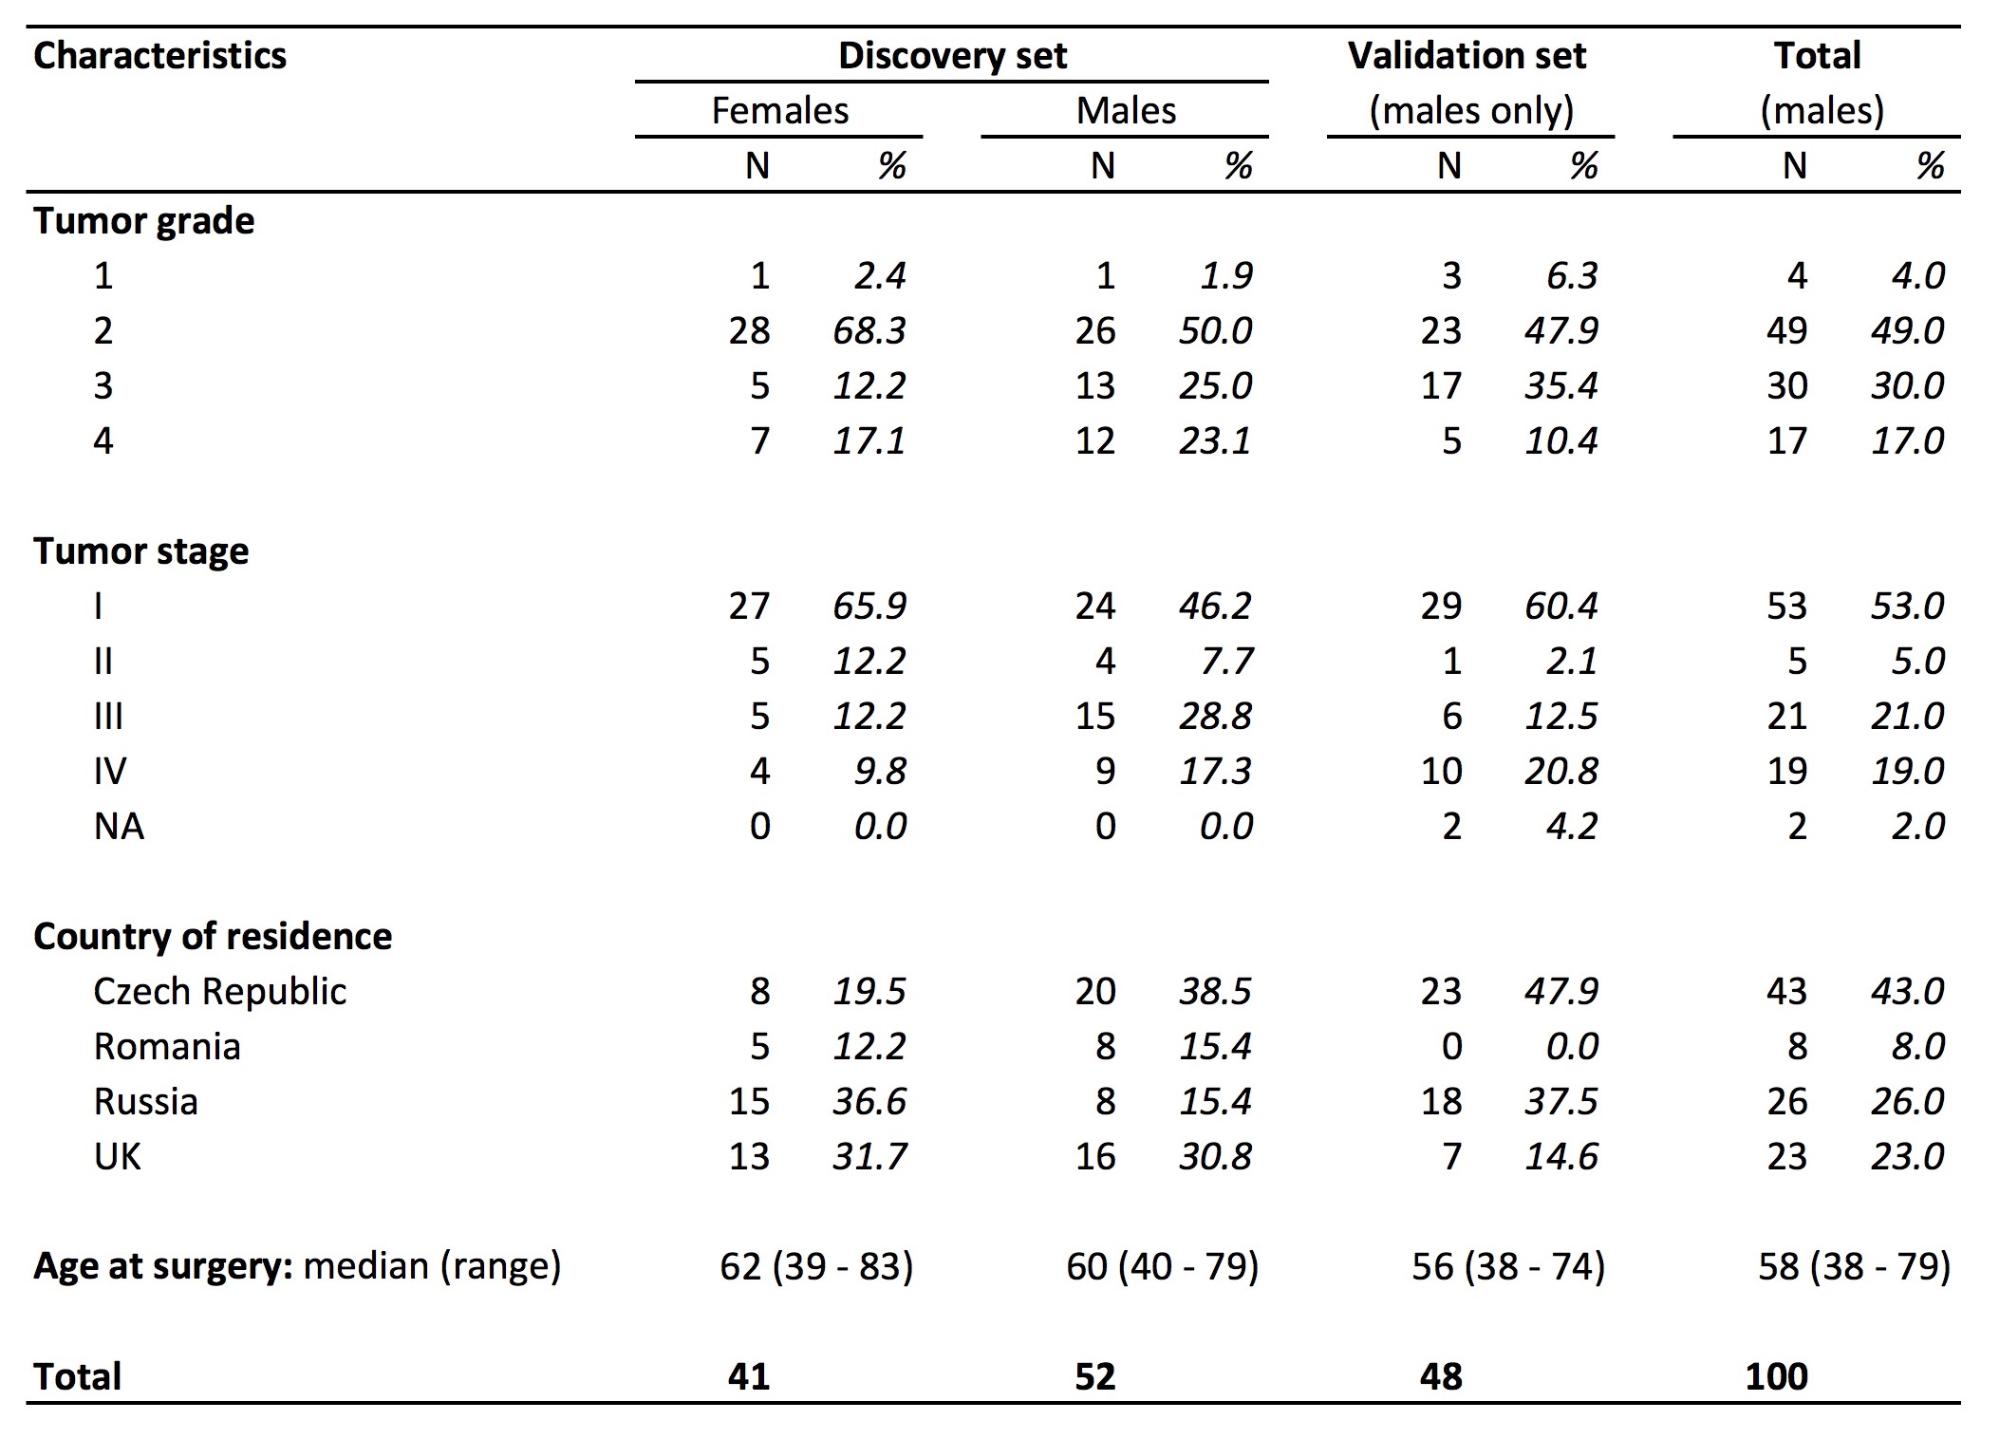
\includegraphics[width=.9\linewidth]{figures/LOY-tabS1.jpg}
  \caption[Characteristics of patients included in the study]{{\bf Characteristics of patients included in the study.}}
  \label{tab:loyS1}
\end{table}

\begin{table}[ht]
  \centering
  \begin{tabular}{lcc}
    Gene           & Chromosome & Fold-change               \\
                   &            & (Differential expression) \\
    \hline
   {\it KDM5D}     & Y          & -1.3                      \\
   {\it USP9Y}     & Y          & -1.4                      \\
   {\it ZFY}       & Y          & -1.1                      \\
   {\it UTY/KDM6C} & Y          & -1.2                      \\
   {\it NLGN4Y}    & Y          & -0.8                      \\
   {\it DDX3Y}     & Y          & -1.8                      \\
   {\it EIF1AY}    & Y          & -1.8                      \\
   {\it TMSB4Y}    & Y          & -0.9                      \\
   {\it RPS4Y1}    & Y          & -2.6                      \\
    \hline
  \end{tabular}
  \caption[Genes differentially expressed between tumors with and without somatic LOY]{{\bf Genes differentially expressed between tumors with and without somatic LOY.} {\small Fold-change of differential expression between the two tumor sets.}}
  \label{tab:loyS2}
\end{table}

\clearpage

\section*{Supplementary Figures}

\begin{figure}[ht]
  \centering
  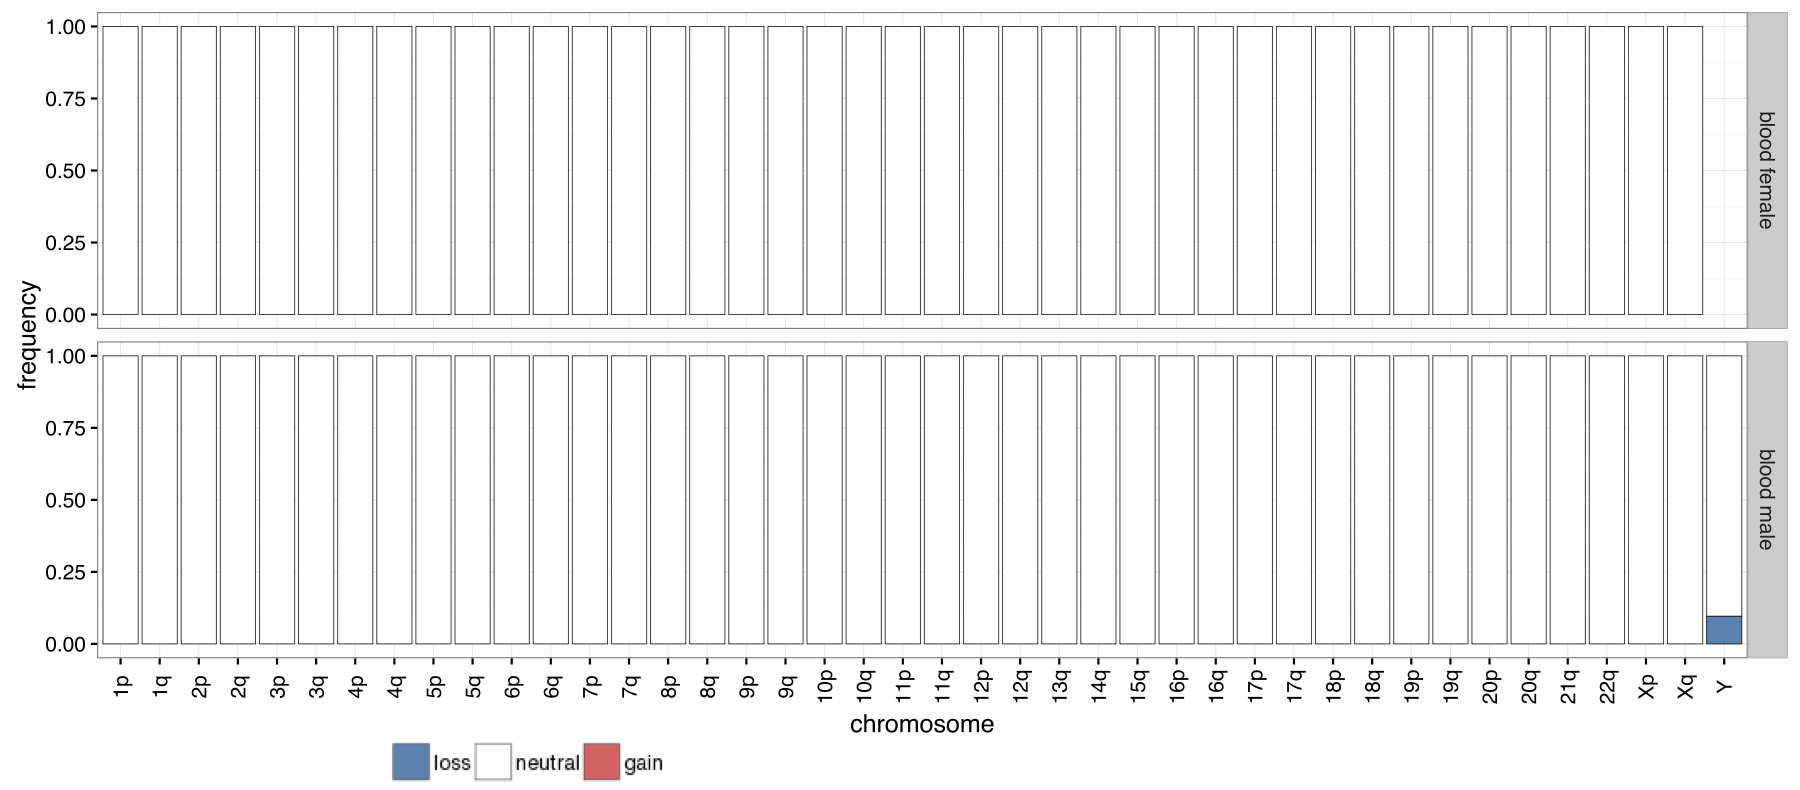
\includegraphics[width=.9\linewidth]{figures/LOY-figS1.png}
  \caption[Copy number analysis in peripheral blood.]{{\bf Copy number analysis in peripheral blood.} {\small Bar graphs show the frequency of copy number variations across the genome in peripheral blood. Frequencies are presented in samples from female and male cases separately.}}
  \label{fig:loyS1}
\end{figure}

\begin{figure}[ht]
  \centering
  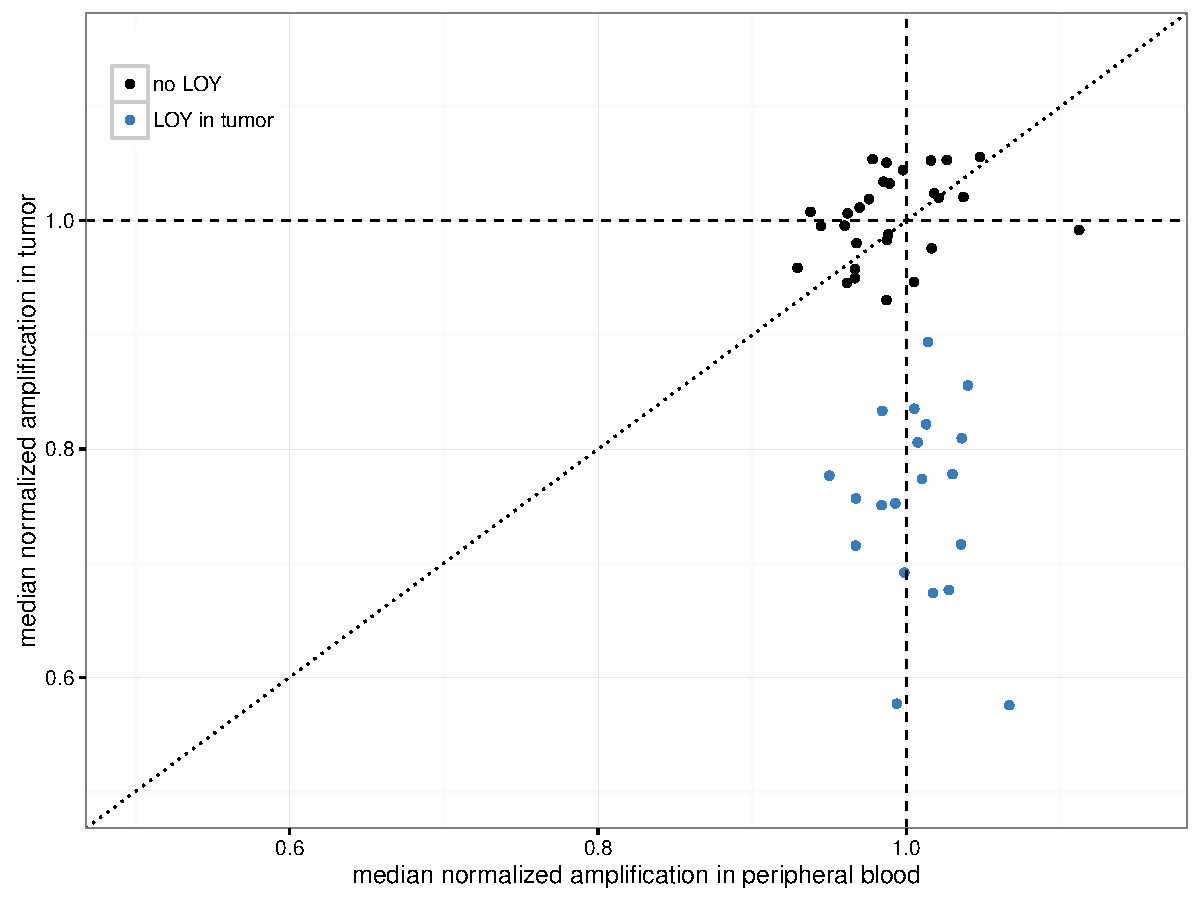
\includegraphics[width=.9\linewidth]{figures/Cagekid-LOY-PCR-fig.pdf}
  \caption[Validation using PCR amplification.]{{\bf Validation using PCR amplification.} {\small Status of chromosome Y in tumors and patient-matched normal samples is shown for individual male subjects of the validation set. The PCR amplification values are normalized and summarized by their median in each sample. Individuals affected by somatic LOY are shown in blue}}
  \label{fig:loyS2}
\end{figure}

\begin{figure}[ht]
  \centering
  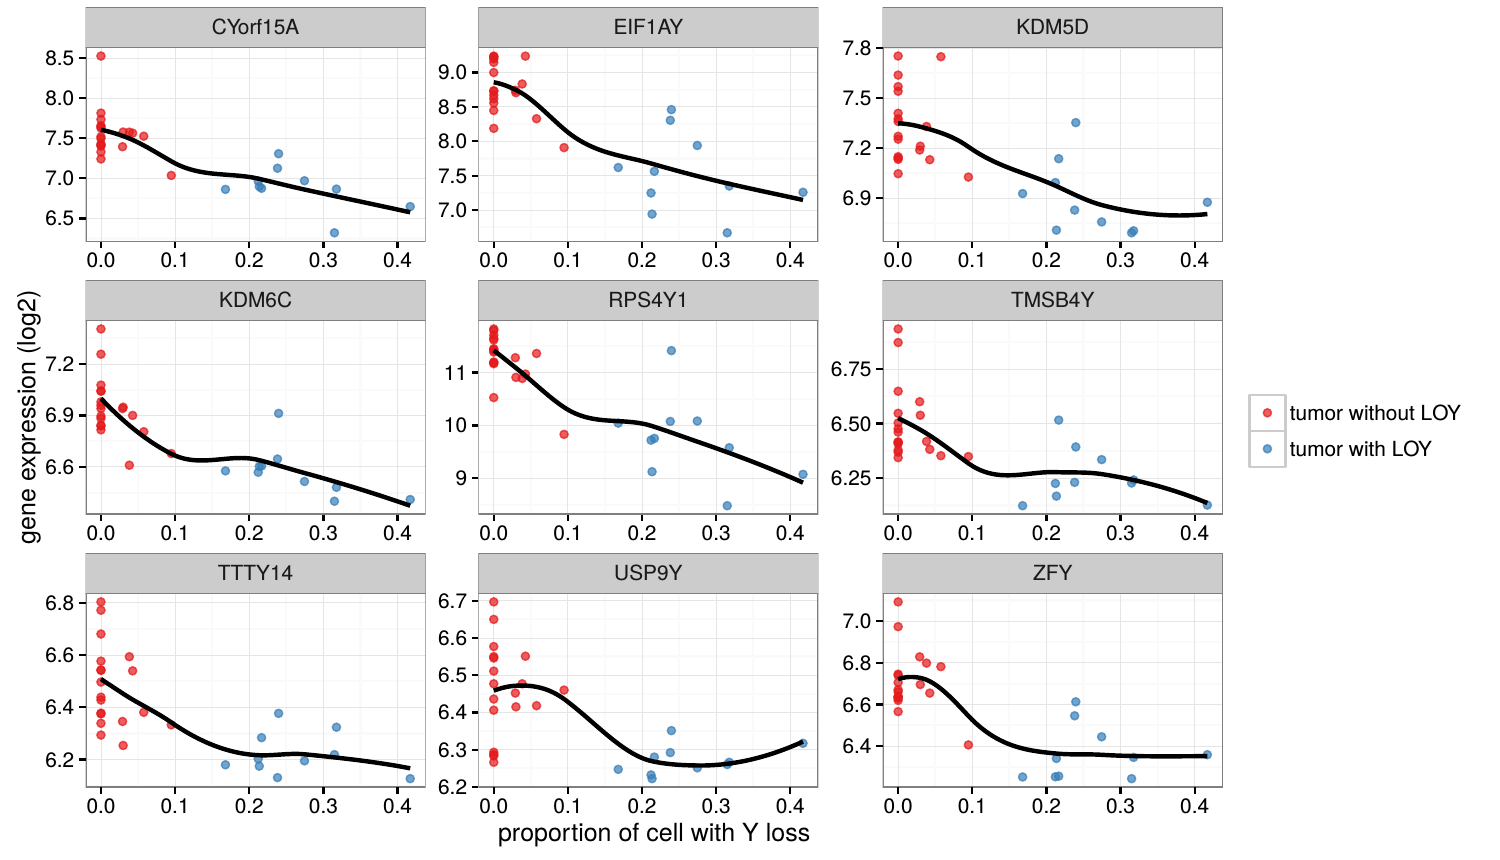
\includegraphics[width=.9\linewidth]{figures/Cagekid-LOY-fig3-array.png}
  \caption[Somatic LOY Y-linked genes down-regulation from array-based expression experiments.]{{\bf Somatic LOY Y-linked genes down-regulation from array-based expression experiments.} {\small The proportion of cells with Y loss was estimated by the PCR amplification values.}}
  \label{fig:loyS3}
\end{figure}

\begin{figure}[ht]
  \centering
  \includegraphics[width=.7\linewidth, page=5]{figures/Cagekid-LOY-fig.pdf}
  \caption[Copy number aberrations of sex chromosomes
and genomic status of X-linked epigenetic modifying genes in tumors of
female and male patients.]{{\bf Copy number aberrations of sex chromosomes
and genomic status of X-linked epigenetic modifying genes in tumors of
female and male patients.} {\small Nearly half of the female tumors harboring
somatic LOX are also affected by mutations of {\it KDM5C}}}
  \label{fig:loyS4}
\end{figure}


\begin{figure}[ht]
  \centering
  \includegraphics[width=.8\linewidth, page=6]{figures/Cagekid-LOY-fig.pdf}
  \caption[Detecting loss of Y.]{{\bf Detecting loss of Y.} {\small The main Gaussian, fitted on the median normalized coverage, is used to detect significant loss/gain. Each male sample, blood and tumor, is colored according to its loss/gain status.}}
  \label{fig:loyS5}
\end{figure}



%%% Local Variables:
%%% mode: latex
%%% TeX-master: "../main"
%%% End:
